\documentclass[12pt,twoside]{report}
\usepackage{graphicx}
\usepackage{alphalph}
\usepackage{subcaption}
\usepackage[a5paper,margin=1cm]{geometry}
\renewcommand*{\thesubfigure}{(\arabic{subfigure})}
\begin{document}
\begin{figure}
\centering
\begin{subfigure}[b]{0.20\textwidth}
\centering

\includegraphics[width=\textwidth]{../../trajectories/104.png}
\caption{Id:104}
\end{subfigure}
\begin{subfigure}[b]{0.20\textwidth}
\centering

\includegraphics[width=\textwidth]{../../trajectories/113.png}
\caption{Id:113}
\end{subfigure}
\begin{subfigure}[b]{0.20\textwidth}
\centering

\includegraphics[width=\textwidth]{../../trajectories/130.png}
\caption{Id:130}
\end{subfigure}
\begin{subfigure}[b]{0.20\textwidth}
\centering

\includegraphics[width=\textwidth]{../../trajectories/717.png}
\caption{Id:717}
\end{subfigure}
\begin{subfigure}[b]{0.20\textwidth}
\centering

\includegraphics[width=\textwidth]{../../trajectories/726.png}
\caption{Id:726}
\end{subfigure}
\begin{subfigure}[b]{0.20\textwidth}
\centering

\includegraphics[width=\textwidth]{../../trajectories/835.png}
\caption{Id:835}
\end{subfigure}
\begin{subfigure}[b]{0.20\textwidth}
\centering
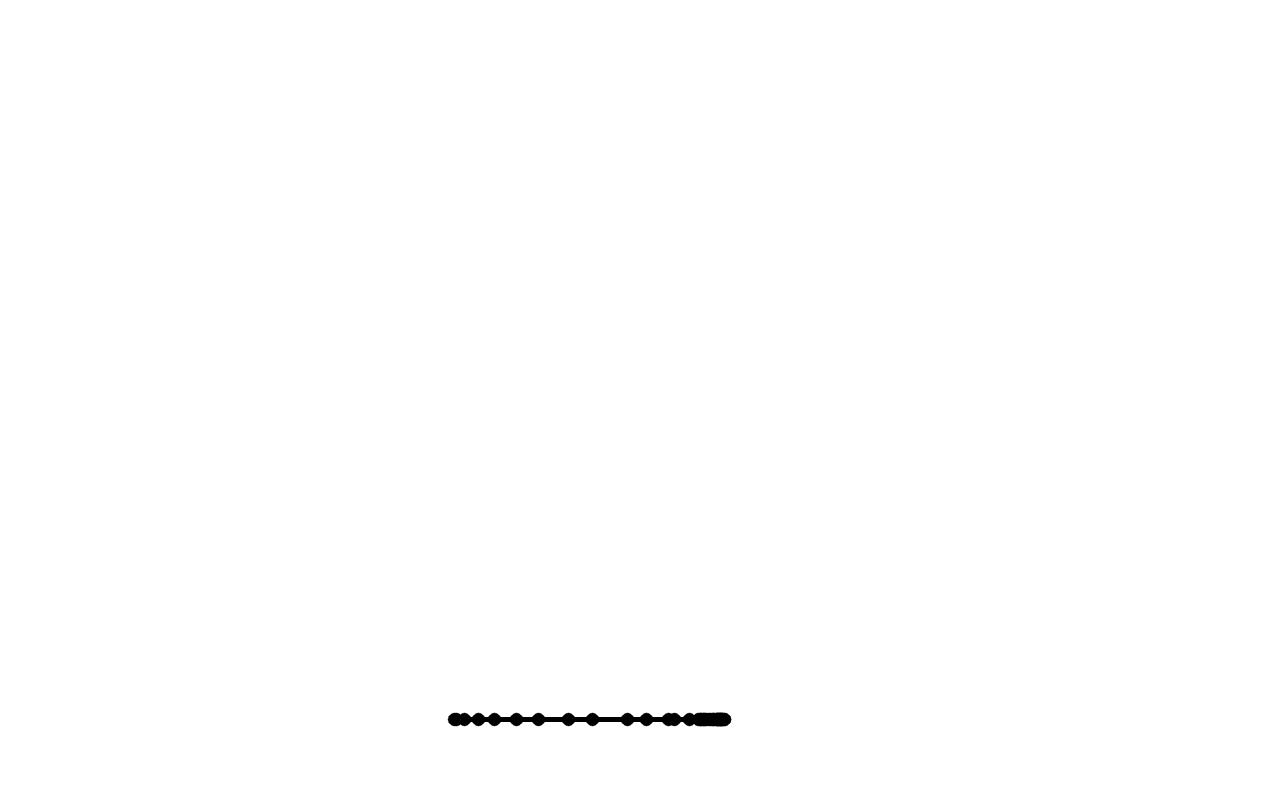
\includegraphics[width=\textwidth]{../../trajectories/836.png}
\caption{Id:836}
\end{subfigure}
\end{figure}
\end{document}